% =====================================================================
%  One-column article template
%  Compile with: pdflatex -> biber -> pdflatex -> pdflatex
%  (or latexmk -pdf main.tex)
% =====================================================================
\documentclass[11pt,a4paper,onecolumn]{article}

% ---------------------------------------------------------------------
%  Page layout & fonts
% ---------------------------------------------------------------------
\usepackage[margin=2.5cm]{geometry}
\usepackage[T1]{fontenc}
\usepackage[utf8]{inputenc}
\usepackage{lmodern}
\usepackage{microtype}
\usepackage{setspace}
\onehalfspacing                 % change to \singlespacing if preferred

% ---------------------------------------------------------------------
%  Mathematics
% ---------------------------------------------------------------------
\usepackage{amsmath,amssymb,amsthm,mathtools}
\usepackage{bm}                 % bold vectors: \bm{x}
\usepackage{siunitx}            % units: \SI{3}{\nano\tesla}
\sisetup{separate-uncertainty=true}

\newtheorem{theorem}{Theorem}
\newtheorem{proposition}{Proposition}
\newtheorem{lemma}{Lemma}
\theoremstyle{definition}
\newtheorem{definition}{Definition}
\theoremstyle{remark}
\newtheorem{remark}{Remark}

% Handy macros
\newcommand{\R}{\mathbb{R}}
\newcommand{\E}{\mathbb{E}}
\newcommand{\vect}[1]{\bm{#1}}
\newcommand{\mat}[1]{\mathbf{#1}}
\DeclareMathOperator*{\argmin}{arg\,min}
\DeclareMathOperator*{\argmax}{arg\,max}

% ---------------------------------------------------------------------
%  Figures, tables, algorithms
% ---------------------------------------------------------------------
\usepackage{graphicx}
\graphicspath{{figures/}}
\usepackage{subcaption}
\usepackage{booktabs}
\usepackage{multirow}
\usepackage[font=small,labelfont=bf]{caption}
\usepackage{algorithm}
\usepackage{algpseudocode}
\usepackage{xcolor}

% ---------------------------------------------------------------------
%  Authors & affiliations
% ---------------------------------------------------------------------
\usepackage{authblk}
\renewcommand\Affilfont{\small}

% ---------------------------------------------------------------------
%  Bibliography (biblatex + biber)
% ---------------------------------------------------------------------
\usepackage[backend=biber,style=numeric-comp,sorting=none,maxbibnames=99]{biblatex}
\addbibresource{references.bib}

% ---------------------------------------------------------------------
%  Hyperlinks & smart references (load last)
% ---------------------------------------------------------------------
\usepackage[colorlinks=true,linkcolor=blue!60!black,citecolor=green!40!black,urlcolor=blue!60!black]{hyperref}
\usepackage[capitalise,noabbrev]{cleveref}

% =====================================================================
%  Title block
% =====================================================================
\title{Title of the Article}

\author[1]{Khaled Surname\thanks{Corresponding author: \texttt{email@ensta.fr}}}
\author[1]{Second Author}
\author[2]{Third Author}
\affil[1]{Lab-STICC, UMR CNRS 6285, ENSTA, Brest, France}
\affil[2]{Other Institution, City, Country}

\date{}  % leave empty, or \today

% =====================================================================
\begin{document}
\maketitle

\begin{abstract}
Write a concise summary (150--250 words): context, problem, proposed
method, main results, and significance.
\end{abstract}

\noindent\textbf{Keywords:} keyword one; keyword two; keyword three; keyword four

% ---------------------------------------------------------------------
\section{Introduction}
\label{sec:intro}
Context and motivation. Related work can be cited like this~\cite{example2024}.
State the contributions clearly:
\begin{itemize}
  \item first contribution;
  \item second contribution;
  \item third contribution.
\end{itemize}
The rest of the paper is organized as follows: \cref{sec:method} presents
the method, \cref{sec:results} the results, and \cref{sec:conclusion} concludes.

% ---------------------------------------------------------------------
\section{Geometry and signal model} \label{sec:setup}

Every channel used in this paper is, to first order, a combination of two fixed functions of one normalised coordinate. this section sets the geometry, derives that coordinate and lists what the platform actually measures.

\subsection{Survey Geometry}\label{subsec:geometry}


The vehicle moves at speed v = 1.0 m/s along straight legs that cross a straight cable at an incidence θ (Figure 1a). Two tri-axial fluxgates are mounted at the water line on the vehicle's lateral axis, UNO on the port side and DUO on the starboard side, separated by the baseline b = 1 m. For each sensor we use a local CPA frame: the origin is the point of its track directly above the cable, x̂ is the horizontal normal to the cable, ŷ points along the cable and ẑ points down (Figure 1b). The cable then lies at x = 0, z = d, where d is the standoff.

A sensor that crosses the cable at time t\textsubscript{c} has horizontal distance x = v(t − t\textsubscript{c}) sin θ from the cable at time t. Every field quantity below depends on x only through the ratio x/d, so we use the normalised coordinate

\[
\tau=\frac{x}{d}=\frac{v\,(t-t_c)\sin\theta}{d}=\frac{t-t_c}{T_s},\qquad T_s=\frac{d}{v\sin\theta}. \tag{1}
\]

τ counts CPA distances, and T\textsubscript{s} is the time the sensor takes to move one CPA distance across the cable; at θ = 50° and v = 1 m/s it is 2.6 s for d = 2 m and 5.2 s for d = 4 m. T\textsubscript{s} is the time scale of every matched template, and we call it the template scale. A leg that starts and ends at the lateral distance A from the cable covers \textbar x\textbar{} ≤ A, i.e.~\textbar τ\textbar{} ≤ K 

with

\[
K=\frac{L}{d},\qquad L=A\ \text{for a snake leg}. \tag{2}
\]

L is the half-length of the pass measured across the cable. With the snake amplitude A = 6 m used in closed loop and d = 2--4 m, K = 3--1.5: a snake leg sees only a few CPA distances on each side of the crossing.

\begin{figure}
\centering

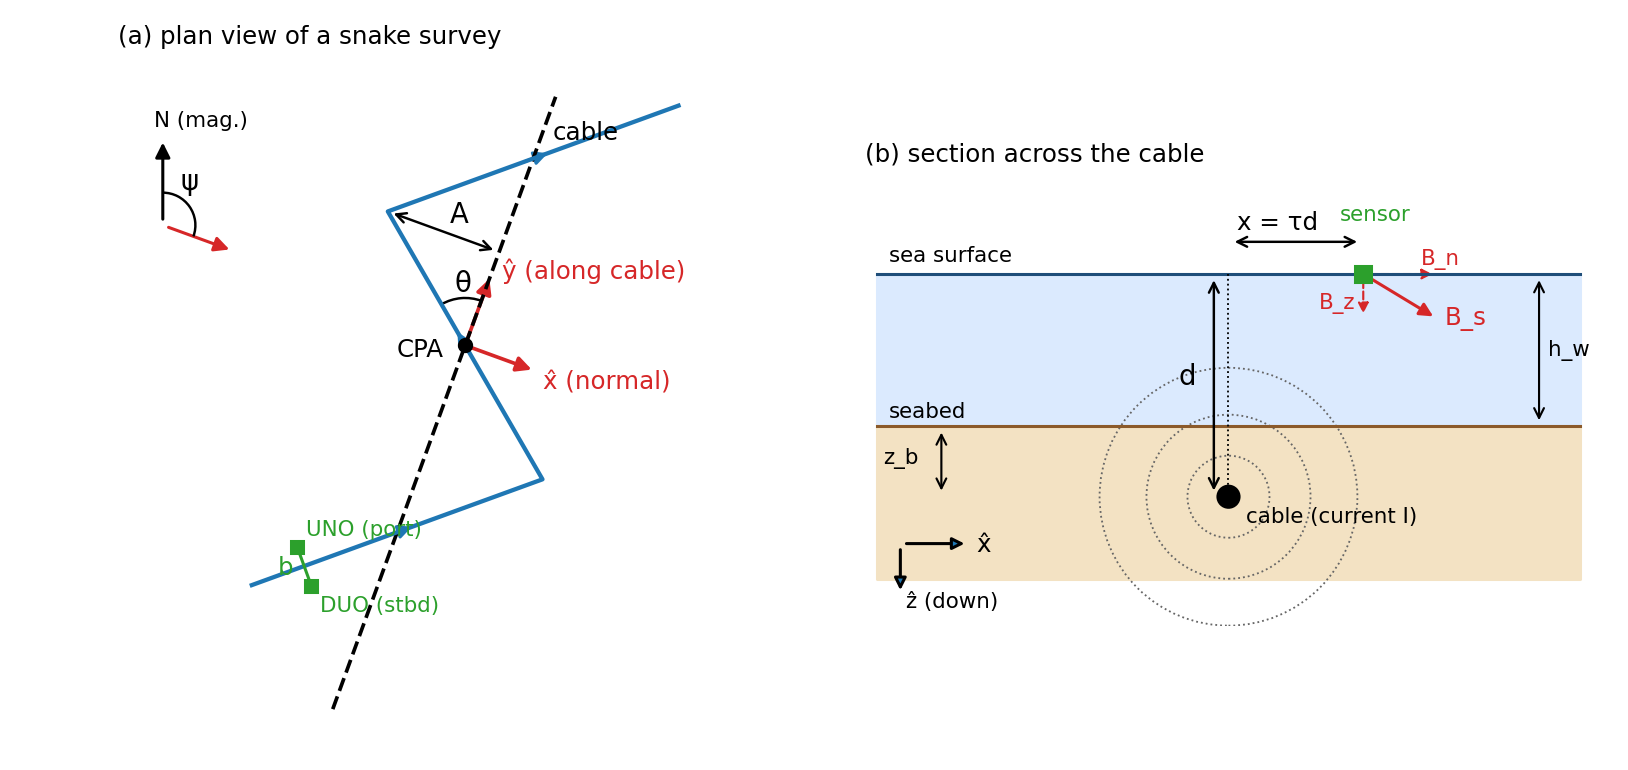
\includegraphics[width=0.98\textwidth,height=\textheight]{paper/sec_2_geometry_signal_model/figures/F1_geometry.png} 

\caption{Survey geometry. (a) Plan view of a snake survey: cable(dashed), legs crossing it at incidence θ with amplitude A, CPA frame (x̂ normal, ŷ along the cable), the two sensors UNO and DUO separated by the baseline b, and the angle ψ from magnetic north to the cable normal. (b) Section across the cable: the sensor at the surface, the cable at standoff d below it (burial depth z\textsubscript{b} below a seabed at water depth h\textsubscript{w}), the normal coordinate x = τd, and the azimuthal cable field B\textsubscript{s} with its normal and vertical components B\textsubscript{n} and B\textsubscript{z}.}
\end{figure}

\subsection{Cable Field and Cable Orthonormal Basis Functions}\label{subsec:cable_obf}

We follow the steps of~\cite{hleis2026obf}. The cable is modeled as an infinitely long straight conductor carrying a DC current $I$, with the return spread through the sea far from the sensor. Its field at the sensor is azimuthal about the cable:
\begin{equation}
    \mathbf{B}_s(\tau) = K_p \left( \frac{1}{1+\tau^2},\; 0,\; \frac{\tau}{1+\tau^2} \right)^{T} = (B_n, B_y, B_z)^{T},
    \qquad K_p = \frac{\mu_0 I}{2 \pi d}.
    \label{eq:cable_field}
\end{equation}
The components are given in the CPA frame: $B_n$ is along the normal $\hat{x}$, $B_y = 0$ is along the cable, and $B_z$ is downwards. $K_p$ is the field magnitude at CPA, $d$ is the standoff distance and $\tau = x/d$ is the normalized along-track position.

The infinite-line model holds when the cable is straight over several standoffs on each side of the crossing. The simulations instead use the exact field of a polyline made of 2~m segments.

Inserting~\eqref{eq:cable_field} into the first-order term of the total-field anomaly gives a sum of two fixed functions of $\tau$. Normalised to unit energy, they are the cable OBF of~\cite{hleis2026obf}:
\begin{equation}
    \Phi_1(\tau) = \sqrt{\frac{2}{\pi}}\,\frac{1}{1+\tau^{2}},
    \qquad
    \Phi_2(\tau) = \sqrt{\frac{2}{\pi}}\,\frac{\tau}{1+\tau^{2}}.
    \label{eq:obf}
\end{equation}
$\Phi_1$ is even and $\Phi_2$ is odd. Both have unit energy over the real line, and they are orthogonal (Appendix~\ref{app:obf_integrals}). The total-field anomaly is then
\begin{equation}
    S(\tau) = A_1 \Phi_1(\tau) + A_2 \Phi_2(\tau),
    \qquad
    A_1 = \sqrt{\frac{\pi}{2}}\,K_p \cos\delta \cos\psi,
    \qquad
    A_2 = \sqrt{\frac{\pi}{2}}\,K_p \sin\delta.
    \label{eq:total_field}
\end{equation}
The factor $\sqrt{\pi/2}$ undoes the normalisation of~\eqref{eq:obf}. $A_1$ and $A_2$ are the coordinates of $S$ in the plane spanned by $\Phi_1$ and $\Phi_2$, and the matched filter of Section~\ref{sec:detection} estimates them. The expansion of the norm that justifies keeping only the first-order term, and the resulting phase, are given in Appendix~\ref{app:total_field_expansion}.

Any channel that is a fixed linear combination of the cable field can be written as one vector of $\mathcal{S} = \mathrm{span}\{\Phi_1, \Phi_2\}$:
\begin{equation}
    s(\tau) = a \left( \cos\beta\, \Phi_1(\tau) + \sin\beta\, \Phi_2(\tau) \right),
    \qquad a \ge 0, \quad \beta \in (-180^{\circ}, 180^{\circ}].
    \label{eq:channel}
\end{equation}

The amplitude $a$ sets the signal level and the phase $\beta$ sets the shape: $\beta = 0$ is the even bell $\Phi_1$, $\beta = 90^{\circ}$ is the odd profile $\Phi_2$, and intermediate phases are asymmetric (Figure~\ref{fig:obf}c).

\paragraph{Hilbert relation.}
The observation underlying this paper is that $\Phi_2$ is the Hilbert transform of $\Phi_1$. The pair is therefore the real and imaginary parts of a single analytic template:
\begin{equation}
    \Phi_2 = \mathcal{H}\{\Phi_1\}, \qquad
    \Psi(\tau) = \Phi_1(\tau) + i\,\Phi_2(\tau) = \sqrt{\frac{2}{\pi}}\,\frac{1}{1 - i\tau},
    \label{eq:analytic}
\end{equation}
and the amplitude and phase of~\eqref{eq:channel} are the modulus and argument of one complex coefficient:
\begin{equation}
    s(\tau) = \Re\left\{ a\,e^{-i\beta}\,\Psi(\tau) \right\}.
    \label{eq:channel_complex}
\end{equation}
This is the line-source instance of the classical property that the horizontal and vertical components of a 2D potential field form a Hilbert pair. Every channel the platform can form is thus one point $a\,e^{i\beta}$ of the complex plane, and the whole paper is an analysis of what each processing step does to that point.

Two properties of $\Psi$ are used (Appendix~\ref{app:analytic_template}). Its spectrum is one-sided, so $\Phi_1$ and $\Phi_2$ have the same autocorrelation. The matched filter of Section~\ref{sec:detection} is then a quadrature receiver, whose output energy is the squared modulus of a single complex correlation and is therefore independent of $\beta$ when the record is unbounded. And $\Psi$ continues analytically off the real axis with a single pole at $\tau = -i$, which is what makes the coherence of a window with the span equal to one at the CPA and nowhere else (Appendix~\ref{app:coherence_uniqueness}). What truncation destroys is the first property, and the displacement it produces is proportional to $\sin 2\beta$.

In the implementation, however, $\Phi_1$ and $\Phi_2$ are used as two real templates and no estimator manipulates complex quantities. The analytic form is a bookkeeping device for the amplitude and the phase.

\paragraph{Gradiometer channels.}
The gradiometer is the difference DUO $-$ UNO. The lateral axis makes the angle $\theta$ with the cable normal, so the two sensors sample the same channel at normal coordinates that differ by $b\cos\theta$, i.e.\ by $h = b\cos\theta/d$ in $\tau$. To first order in that difference (a central difference),
\begin{equation}
\begin{gathered}
\Delta s(\tau) \simeq \frac{b\cos\theta}{d}\,\frac{\mathrm{d}s}{\mathrm{d}\tau}
= \frac{b\cos\theta}{\sqrt{2}\,d}\,a\left(\cos\beta\,\Gamma_1(\tau) + \sin\beta\,\Gamma_2(\tau)\right),\\[2pt]
\Gamma_1 = \sqrt{2}\,\Phi_1' = -\frac{4}{\sqrt{\pi}}\frac{\tau}{(1+\tau^{2})^{2}},
\qquad
\Gamma_2 = \sqrt{2}\,\Phi_2' = \frac{2}{\sqrt{\pi}}\frac{1-\tau^{2}}{(1+\tau^{2})^{2}}.
\end{gathered}
\label{eq:grad_obf}
\end{equation}
The factor $\sqrt{2}$ makes $\Gamma_1$ and $\Gamma_2$ unit-energy: with the integrals of Appendix~\ref{app:obf_integrals} and $(1-\tau^{2})^{2} = (1+\tau^{2})^{2} - 4\tau^{2}$,
\[
\int \Phi_1'^{\,2} = \frac{2}{\pi}\int\frac{4\tau^{2}}{(1+\tau^{2})^{4}} = \frac{1}{2},
\qquad
\int \Phi_2'^{\,2} = \frac{2}{\pi}\left(\int\frac{\mathrm{d}\tau}{(1+\tau^{2})^{2}} - 4\int\frac{\tau^{2}}{(1+\tau^{2})^{4}}\right) = \frac{1}{2}.
\]
$\Phi_1'$ is odd and $\Phi_2'$ is even, so $\Gamma_1$ and $\Gamma_2$ are orthogonal by parity (Figure~\ref{fig:obf}b): the vertical gradiometer $\Delta B_z$ follows the even profile $\Gamma_2$ and the horizontal gradiometer follows the odd profile $\Gamma_1$. Since $B_y = 0$ everywhere, the horizontal cable field points along $\hat{x}$ at both sensors, and so does their difference: the horizontal gradiometer vector lies along the cable normal. The first-order model~\eqref{eq:grad_obf} follows from $s(\tau + h/2) - s(\tau - h/2) = h\,s'(\tau) + (h^{3}/24)\,s'''(\tau) + O(h^{5})$, so its relative error is of order $h^{2}/24$ times the ratio of the third to the first derivative.

The gradiometer amplitude is reduced by $b|\cos\theta|/(\sqrt{2}\,d)$, and it vanishes at perpendicular incidence.

The channels of this paper have the following amplitudes and phases (with $K' = \sqrt{\pi/2}\,K_p$):

\begin{table}[H]
\centering
\small
\caption{Amplitude and phase of each channel in the basis $\{\Phi_1, \Phi_2\}$.}
\label{tab:channels}
\begin{tabular}{@{}%
  >{\raggedright\arraybackslash}p{0.36\linewidth}%
  >{\raggedright\arraybackslash}p{0.28\linewidth}%
  >{\raggedright\arraybackslash}p{0.28\linewidth}@{}}
\toprule
Channel & Amplitude $a$ & Phase $\beta$ \\
\midrule
Normal component $B_n$
  & $K'$
  & $0$ \\
Vertical component $B_z$
  & $K'$
  & $90^{\circ}$ ($-90^{\circ}$ for the opposite current) \\
North and East components, $B_n\cos\psi$ and $B_n\sin\psi$
  & $K'|\cos\psi|$, $K'|\sin\psi|$
  & $0$ or $180^{\circ}$ \\
Total field $S$
  & $K'\sqrt{\cos^{2}\delta\,\cos^{2}\psi + \sin^{2}\delta}$
  & $\tan\beta = \tan\delta / \cos\psi$ \\
Gradiometer, horizontal normal $\Delta B_n$
  & $\dfrac{K'\,b\,|\cos\theta|}{\sqrt{2}\,d}$
  & $0$ on the gradiometer basis (odd profile $\Gamma_1$) \\
Gradiometer, vertical $\Delta B_z$
  & $\dfrac{K'\,b\,|\cos\theta|}{\sqrt{2}\,d}$
  & $90^{\circ}$ on the gradiometer basis (even profile $\Gamma_2$) \\
\bottomrule
\end{tabular}
\end{table}

The vector components have phases fixed by physics. The total-field phase follows from~\eqref{eq:total_field}, $\tan\beta = A_2/A_1 = \tan\delta / \cos\psi$ (Appendix~\ref{app:total_field_expansion}). Since $|\cos\psi| \le 1$, we have $|\tan\beta| \ge \tan\delta$, so $\beta$ lies between $\delta$ and $180^{\circ} - \delta$: between $63.7^{\circ}$ and $116.3^{\circ}$ at Brest, for every cable bearing. The total field is therefore always closer to the odd profile than to the even one. At $\psi = 45^{\circ}$, for example, $\beta = 70.7^{\circ}$.

\begin{figure}[t]
\centering
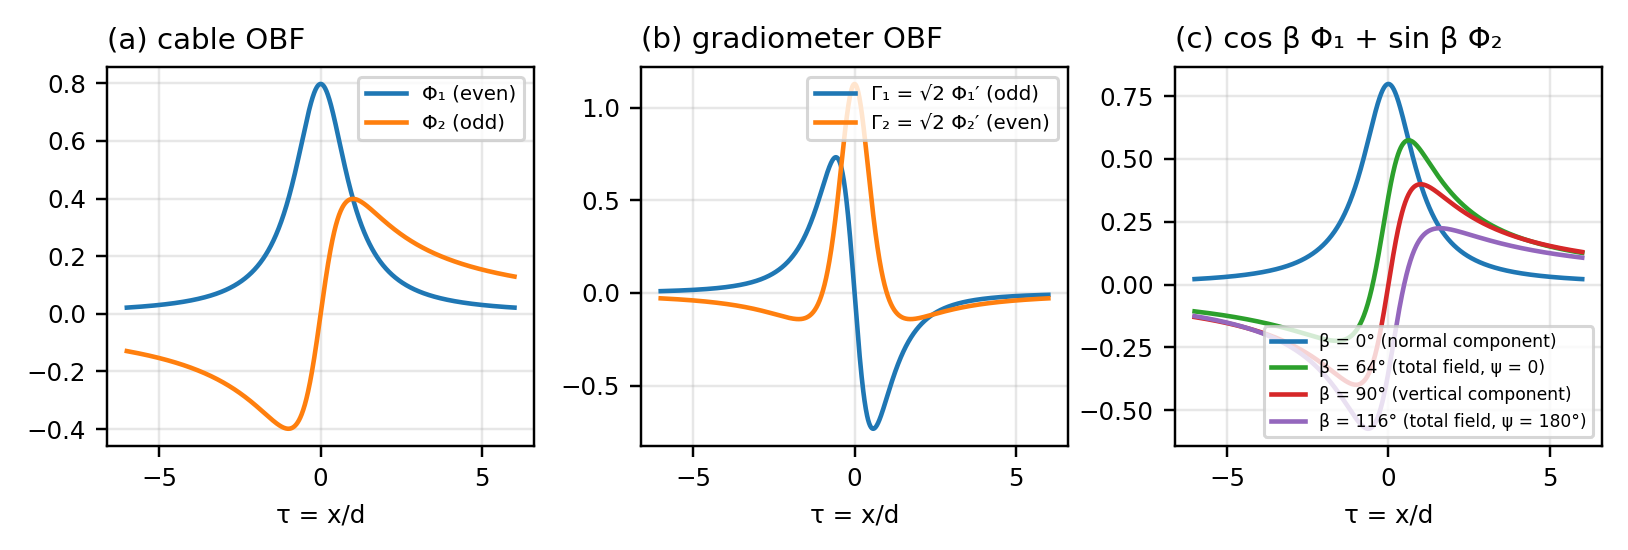
\includegraphics[width=\linewidth]{paper/sec_2_geometry_signal_model/figures/F2_bases.png}
\caption{(a) Cable OBF: the even $\Phi_1$ and the odd $\Phi_2$ of~\eqref{eq:obf}.
(b) Gradiometer OBF: the odd $\Gamma_1$ and the even $\Gamma_2$ of~\eqref{eq:grad_obf}.
(c) Channels of~\eqref{eq:channel} for $\beta = 0^{\circ}$ (normal component), $90^{\circ}$ (vertical component), and the limits $64^{\circ}$ and $116^{\circ}$ of the total-field phase at Brest.}
\label{fig:obf}
\end{figure}

\subsection{What the Platform Measures}\label{subsec:signal_model}

Each body-mounted sensor records the body-frame vector
\begin{equation}
    \vect{F}_b = (\mat{I} + \mat{E}_s)\,\mathbf{R}^{nb}(\mathrm{roll},\mathrm{pitch},\chi)\,(\vect{T} + \vect{B}_s + \vect{B}_{ext}) + \vect{h}_s + \vect{n}_s.
    \label{eq:recorded_field}
\end{equation}
Here $\vect{B}_{ext}$ is an external magnetic field that is not the cable anomaly, and $\mat{E}_s$ and $\vect{h}_s$ are the soft-iron matrix and the hard-iron offset left after sensor calibration, which also absorb the static field of the platform that calibration did not account for.
$\mathbf{R}^{nb}$ is the rotation matrix from the NED frame to the body frame, with $\chi$ the yaw of the vehicle, and applying it requires the attitude to be known.
$\vect{n}_s$ is the sensor noise.

Three channels are formed from the recorded field.
\begin{itemize}
    \item \textbf{Total field} $|\vect{F}_b|$. This channel is the norm of the measured components. Its main advantage is its independence from the attitude, so the errors of attitude estimation are absent.
    \item \textbf{Vector components in NED.} Contrary to \todo{[2]}, the processing is done in the NED frame, so the data are expressed in a frame that follows the vehicle but whose rotation is locked to north and east. Removing the regional field depends on the attitude estimate, which leaks an error from the regional field into the components that is comparable to the cable anomaly in this channel. This effect is tested in the later sections.
    \item \textbf{Gradiometer DUO $-$ UNO.} $\vect{T}$ and $\vect{B}_{ext}$ are common to both sensors and cancel, so an attitude error then rotates only the difference vector. The attitude is still needed to orient the measurements in NED before the difference is taken.
\end{itemize}

The total field needs no attitude but mixes the two phases, so its shape changes with $\beta$.
The vector components have a pure phase, so their shape does not vary with $\beta$, but they need the attitude.
The gradiometer also has a pure phase and needs only the heading from the attitude, at the cost of an amplitude reduced by the factor $b|\cos\theta|/(\sqrt{2}\,d)$.
This trade-off organises every comparison that follows.

% ---------------------------------------------------------------------
\section*{Acknowledgments}
Funding sources and acknowledgments.

\section*{Data Availability}
Statement on data and code availability.

% ---------------------------------------------------------------------
\printbibliography[heading=bibintoc,title={References}]

% ---------------------------------------------------------------------
\appendix
\section{Proof or Additional Derivations}
\label{app:proof}
Supplementary material.

\end{document}